%https://en.wikibooks.org/wiki/LaTeX/Mathematics
\newcommand{\ignore}[1]{}
\documentclass[12pt]{article}
\usepackage{placeins}
\usepackage[left]{lineno}
%\linenumbers  THIS TERRIBLE BUGY!
\usepackage{amsmath}
\usepackage{amssymb}
\usepackage{cancel}
 \usepackage{graphicx}
\usepackage{braket}
\usepackage{authblk}
\usepackage{caption,subcaption}
\usepackage{comment}
\usepackage{enumitem}
\usepackage[utf8]{inputenc}
%\usepackage{subfigure}
\usepackage[pdftex, pdfstartview={FitH}, pdfnewwindow=true, colorlinks=false, pdfpagemode=UseNone]{hyperref}
\numberwithin{equation}{section}
\numberwithin{figure}{section}
\graphicspath{{fig/}}
\setlength{\parskip}{.2in}
\setlength{\parindent}{.4 in}
\renewcommand{\baselinestretch}{1.1}
\setlength{\topmargin}{-.3in} \setlength{\oddsidemargin}{.0in}
  %\setlength{\evensidemargin}{-.21in}
\setlength{\textheight}{8.5in} \setlength{\textwidth}{6.35in}
  \setlength{\footnotesep}{\baselinestretch\baselineskip}
  \newlength{\abstractwidth}
  \setlength{\abstractwidth}{\textwidth}
  \addtolength{\abstractwidth}{-6pc}

% To only number one line of a multi-line eqn.
\newcommand\numberthis{\addtocounter{equation}{1}\tag{\theequation}}

\usepackage[usenames,dvipsnames,svgnames,table]{xcolor}
\newcommand{\rcb}[1]{\textcolor{blue}{  #1 }}
\newcommand{\esw}[1]{\textcolor{violet}{  #1 }}
\newcommand{\com}[1]{\textcolor{red}{  #1 }}
\newcommand{\be}{\begin{equation}}
%\newcommand{\be}{\begin{linenomath}}
 \newcommand{\ee}{\end{equation}}
%\newcommand{\ee}{\end{linenomath}}
\newcommand{\bea}{\begin{eqnarray}}
\newcommand{\eea}{\end{eqnarray}}
\newcommand{\beq}{\begin{equation}}
\newcommand{\eeq}{\end{equation}}
  \newcommand{\N}{{\cal N}}
  \newcommand{\<}{\langle\,}
  \newcommand{\oc}{{\cal O}_C}
  \renewcommand{\a}{\alpha}
  \renewcommand{\b}{\beta}
  \newcommand{\half}{{\small 1\over 2}}
  \renewcommand{\>}{\rangle}
\newcommand\dd{\partial}
\newcommand\nn{\nonumber \\}
\newcommand\mD{{\mathbb D}}
\newcommand\mS{{\mathbb S}}
\newcommand\mR{{\mathbb R}}
\newcommand\mT{{\mathbb T}}
\newcommand\mEye{{\mathbb I}}
\newcommand\cO{{\cal O}}
\renewcommand\ell{l}
\newcommand\levec[1]{\langle #1 |}
\newcommand\revec[1]{| #1 \rangle}
\newcommand\rbj{\mbox{\scriptsize rbj}}

% set footnotes to symbols, not numbers
\renewcommand*{\thefootnote}{\fnsymbol{footnote}}

\newcommand*\Laplace{\mathop{}\!\mathbin\bigtriangleup}
\newcommand\onehalf{\frac{1}{2}}
\newcommand{\ndim}[1]{#1-d}
\newcommand{\eqn}[1]{Eq.~\ref{#1}}
\usepackage{placeins}

%Evan new commands!
\newcommand{\spinup}{\binom{1}{0}}
\newcommand{\spindown}{\binom{0}{1}}
\newcommand\Pm{P_-}
\newcommand\Pp{P_+} 
\newcommand\Pmg{\mathbb{P}}
\newcommand{\blue}[1]{\textcolor{blue}{#1}}
\newcommand\BNO{{\tt BNO}}

%\usepackage[inline]{showlabels}
%\showlabels{cite} 

\def\bfs{{\color{red} \bf COMMENT:} \color{blue}}
\title{Continuous Time SW Algorithm}

\author[*]{Richard C. Brower}
%\affil[*]{Boston University, Boston, MA 02215, USA}xi

\date{\today}

\begin{document}

\maketitle

\section{Introduction}

The paper ( \href{https://arxiv.org/abs/cond-mat/9802104v1}{https://arxiv.org/abs/cond-mat/9802104v1}   on {\bf Application of a continuous time cluster algorithm to the Two-dimensional Random Quantum Ising Ferromagnet} by Heiko Rieger and  Naoki Kawashima has the correct formulation but  lack details for write code

The paper does the Swendsen Wang update in the limit of zero time
lattice spacing, $a_t$,
for any Ising Hamiltonian on a spacial graph in 4 cycles illustrated
in Fig.\ref{fig:ABCD}

The partition function
\be
Z = \sum_{s_i = \pm 1} e^{\textstyle  K^0_{t,i}  s_{t,i}   s_{t+1,i} + \sum_{\<i,j\>} \widetilde K^\perp_{ij} s_{t,i}   s_{t,j}} 
\ee
becomes 
\be
Z =Tr[ e^{ -  \beta \hat H} ] \quad \mbox{where} \quad  \hat H   = - \sum_i \Gamma_i
\sigma^x_i -  \sum_{\<i,j\>}  J_{ij} \sigma^z_i \sigma^z_j 
\ee
in the limit $a_t \rightarrow 0$  with $\widetilde K^\perp_{ij} = a_t  J_{ij}$ and $e^{ - 2 a_t K_i} = \tanh(a_t \Gamma_i)$.

\begin{figure}[h]
    \centering
    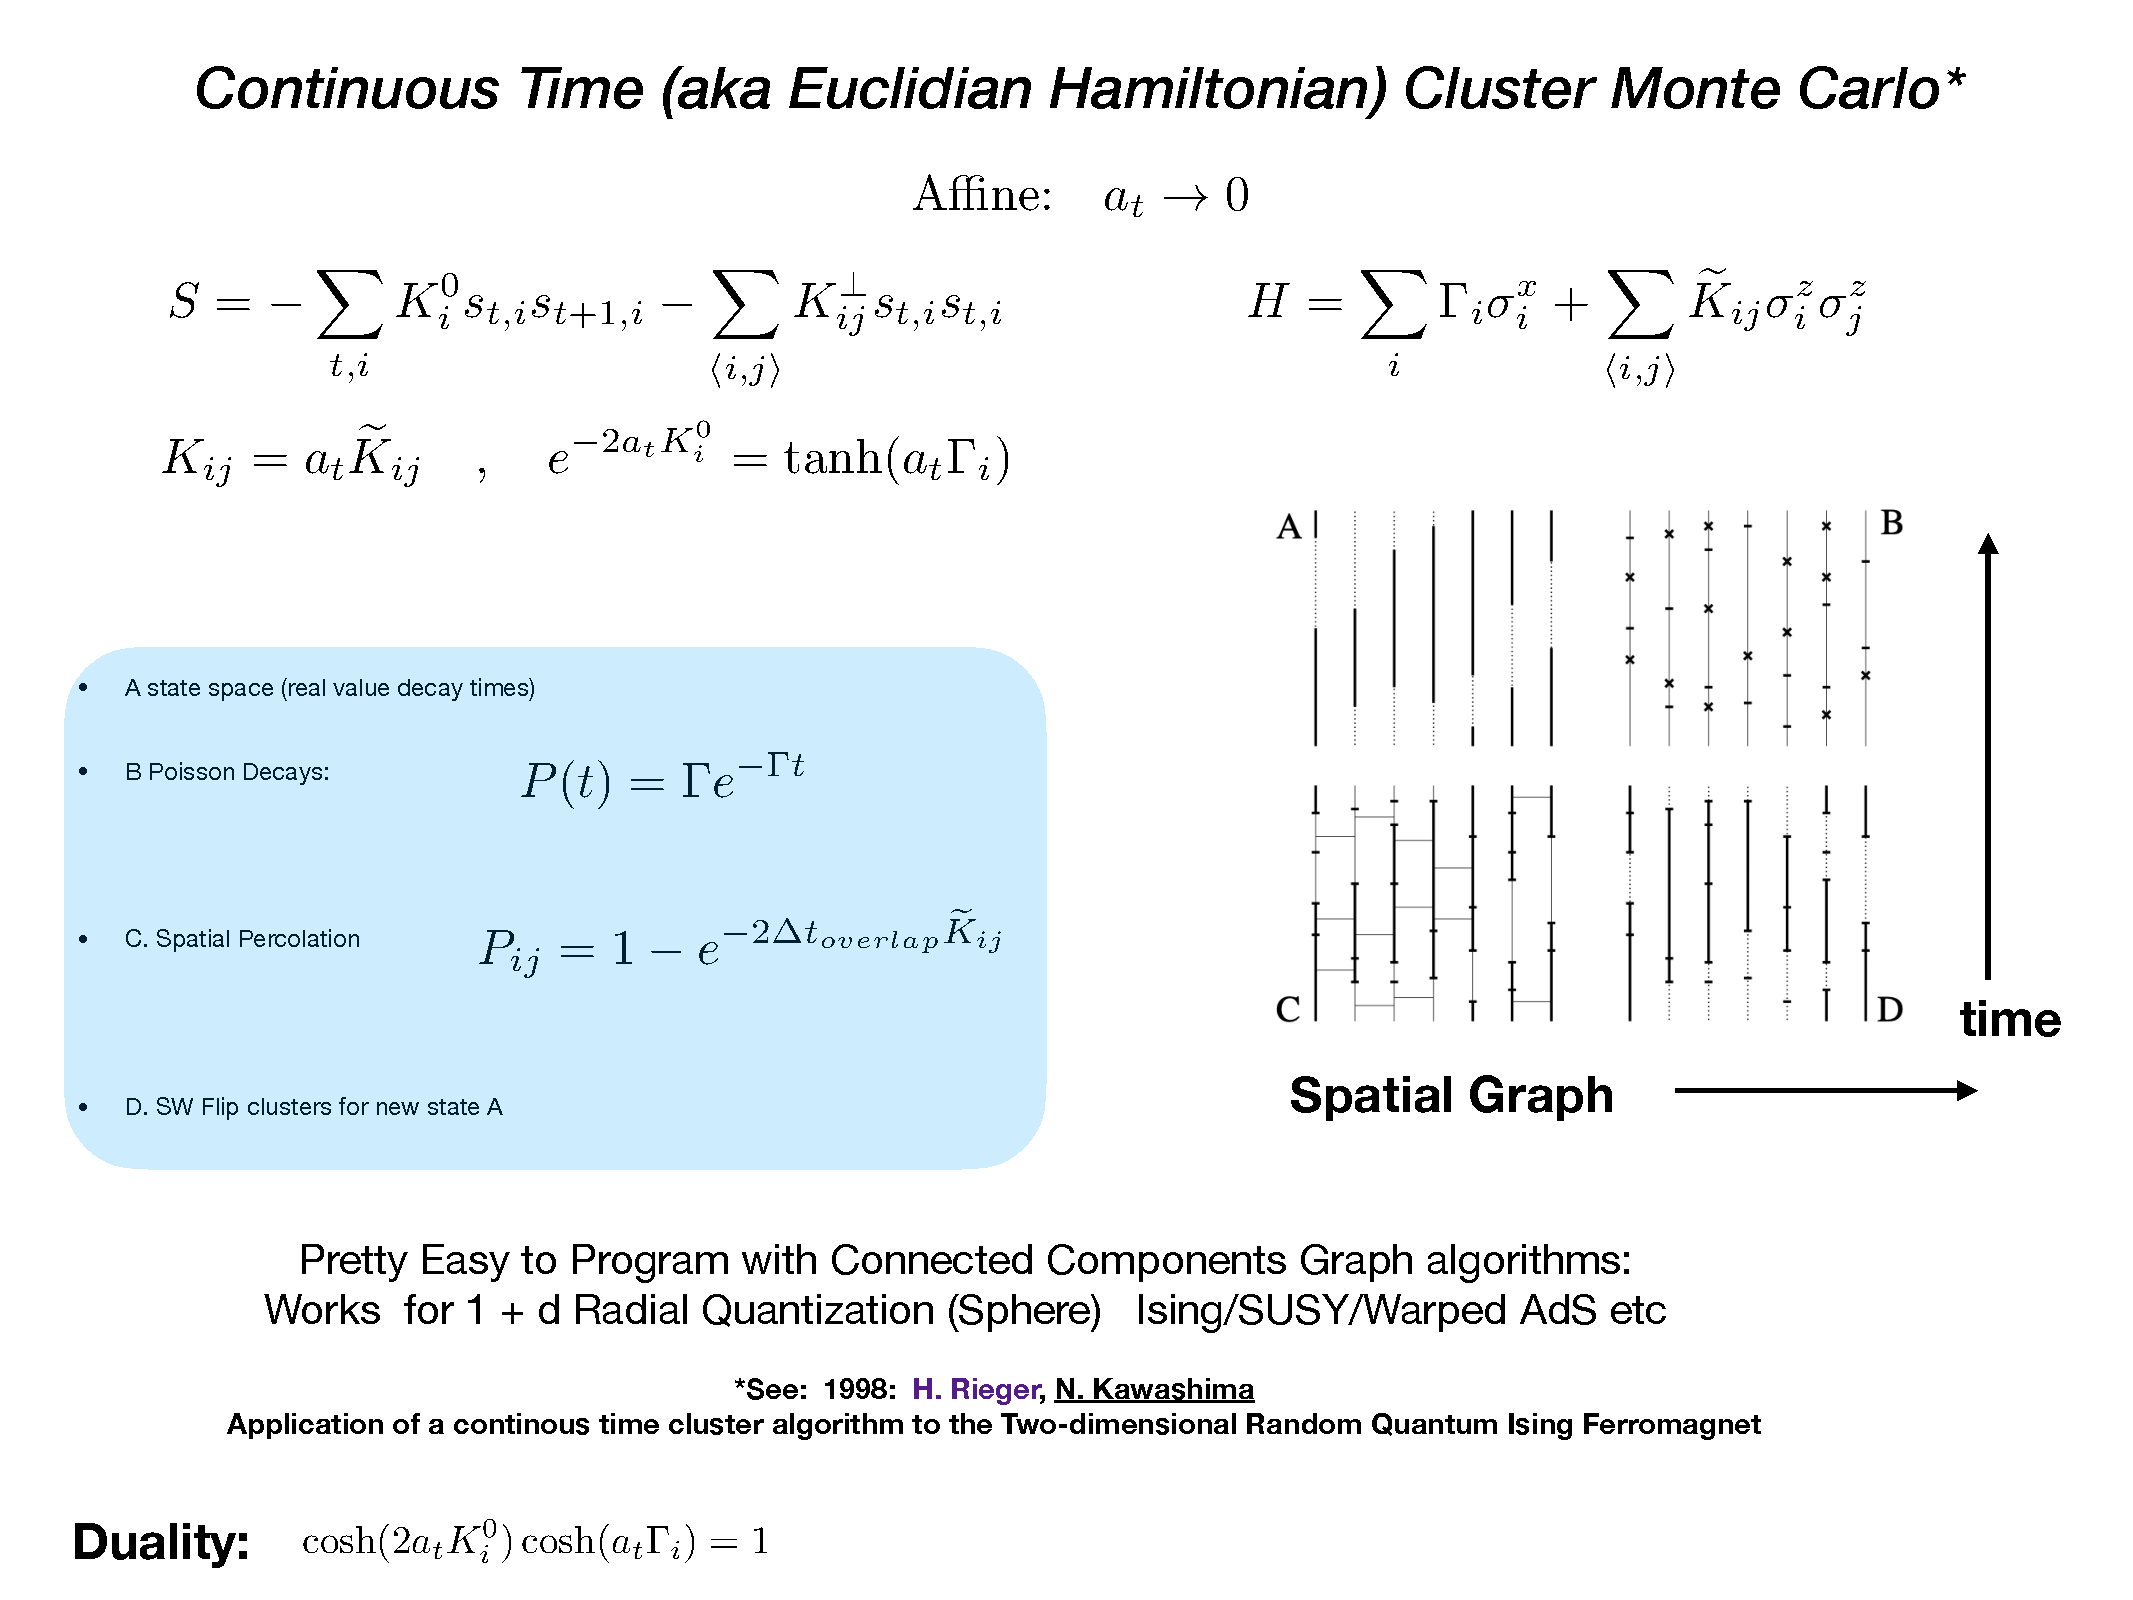
\includegraphics[width=1.1\textwidth]{QuLat_Jan_2024_final}
    \caption{Slide from QuLAT meeting Jan 2024. I switch to Heiko Rieger and  Naoki Kawashima notation: $J_{ij} = \widetilde K_{ij}$. }
    \label{fig:ABCD}
  \end{figure}
  
\section{Formalism}


The state space is A in figure. It is a sequence of broken bounds at
$0 < t_i \le \beta$ in vertical lines.  The number of broken  of bonds
(i.e decays sequence) in time $ \Delta t$ is the Poisson distribution $n =  0,1,2, \cdots, \infty$ 
\be
p_n  =\frac{ \lambda^n e^{ \textstyle - \lambda}}{n!} 
\ee
with $\lambda =  \Delta t \Gamma$.
\href{https://en.wikipedia.org/wiki/Poisson\_distribution}{https://en.wikipedia.org/wiki/Poisson\_distribution}
This is equivalent to a decay rate $P(t) = \Gamma \exp[ -t \Gamma]$, normalized to  $\int^\infty_0 P(t) = 1$ with mean lifetime:
\be
\int^\infty_0 dt \;   t  \; \Gamma e^{\textstyle - t \Gamma} = 1/\Gamma
\ee


The probability of no decay in interval $[0,\Delta t ]$ is 
\be
p_0 = \Gamma \int^\infty_{\Delta t}   e^{\textstyle - t \Gamma}   =
e^{\textstyle - \Gamma \Delta t}
\ee

Theorem: The distribution of  n decay time in an interval $\Delta t $ for n -decay is
a random series of times: $t_0 = 0 < t_1 < t_2 < \cdots<  t_n < \Delta t $.
The Poisson distribution is give by both by the time ordered sequence of
 decays in  intervals $0<\Delta t_i = t_i - t_{i-1}< \Delta t$ {\bf and} the
uniform distribution random times in $[ 0,\Delta t]$:
\bea
p_n &=&  \int^{\Delta t}_{t_{n-1}} dt_n  \cdots  \int^{\Delta t_2}_{0} dt_1  (\Gamma e^{\textstyle  - \Delta t_1 \Gamma}) 
\times \cdots \times  ( \Gamma e^{\textstyle  - \Delta t_n\Gamma}) \times ( e^{\textstyle  - (\Delta
  t -   [ \Delta t_1+ \cdots + \Delta t_n]) \Gamma}) \nn
&=&  \int^{\Delta t}_{t_{n-1}} dt_n  \cdots  \int^{\Delta t_2}_{0} dt_1  \Gamma^n e^{\textstyle  - \Delta t \Gamma} = \frac{1}{n!} (\prod_i \int^{\Delta t}_0 dt_i ) \; \Gamma^n e^{\textstyle - \Delta t \Gamma}  =   \frac{ (\Delta t \Gamma)^n e^{\textstyle - \Delta t \Gamma} }{n!} 
\eea
This allows us to introduce cut links as sequence of decays in any interval until we run out
of space! Very efficient algorithm going for stage A to B.

The step form B to C constructs new cluster with percolation in to
neighboring links with probability
\be
p_{\<i,j\>} = e^{\textstyle - 2 J_{ij} \Delta t_{ij}}
\ee
where $\Delta t_{ij}$ is the overlap time interval between equal spin
segments on the $\<i,j\>$ edges.




\section{ Data Structures}

The state is keep in a basic Data struture, called Rails.The
`Langrangian''  phase space for the partion funtion $Z = Tr[ e^ {
  -\beta  H}] $ are strips of Euclidean time length $DetlaT = \beta$ with
cut-bonds at each spacial site $x = 0\cdots  L-1$. The state is keep in
a basic Data struture, called Rails.
\begin{verbatim}
struct param{
  double  DeltaT;
  double Gamma;
  int N;
  vector<double>  time[L];
  vector<int>  spin[L];
  vector<int> clusterNumber[L];
};
\end{verbatim}
Rail for each $x = 0,\cdots, L-1$ is  a  list of times and corresponding spins 
\be
t_i = {\sc time}[x][i]  \quad, \quad s_i = {\sc spin}[x][i] \in \{t_{I+1}, t_i\}
\ee
 The spins are assigne to each interval:
\be
t_0 = 0 < t_1 <  t_2< \cdot < t_n <  t_{n+1} = T 
\ee 
between the cuts at $t_i$ for $i = 0,..,n$. 
{\bf Perodic B.C are enforced}  ``removing the virtual cut at $t = 0$
and $t = T$ are glued together by  joining the first and last strip  with single spin
\be
s_0 = s_n \in \{T, t_n\} \cup  \{t_1, 0\}
\ee
If you don't do this you can have fixed Dirichlet boundary condition by fixing
$s_0, s_n$ or Neumann by letting theme be independent variable.

All the steps A,B,C and D update in place this data structure!









\end{document} 